% =====================================================================
%  English Writing & Presentation Skills
%  Topic: Describe a project which you have worked on
%  Project: Course Management & Registration System
%  Compile: pdflatex report.tex      (maximum length: 6 pages)
% =====================================================================
\documentclass[12pt,a4paper]{article}

\usepackage[utf8]{inputenc}
\usepackage[T1]{fontenc}
\usepackage{lmodern}
\usepackage[margin=2.2cm,headsep=0.6cm]{geometry}
\usepackage{setspace}
\usepackage{xcolor}
\usepackage{titlesec}
\usepackage{enumitem}
\usepackage{booktabs}
\usepackage{tabularx}
\usepackage{array}
\usepackage{tikz}
\usetikzlibrary{positioning,arrows.meta}
\usepackage{fancyhdr}
\usepackage{caption}
\usepackage{float}
\usepackage[hidelinks]{hyperref}

% ---------- Fill in your details here ----------
\newcommand{\studentname}{Your Full Name}
\newcommand{\studentid}{Student ID}
\newcommand{\coursename}{English Writing \& Presentation Skills}
\newcommand{\lecturer}{Lecturer's Name}
% -----------------------------------------------

\definecolor{primary}{HTML}{1F4E5F}
\definecolor{accent}{HTML}{E07A2F}

\titleformat{\section}{\Large\bfseries\color{primary}}{\thesection.}{0.6em}{}
\titleformat{\subsection}{\large\bfseries\color{primary}}{\thesubsection}{0.6em}{}
\titlespacing*{\section}{0pt}{1.1em}{0.4em}
\titlespacing*{\subsection}{0pt}{0.7em}{0.3em}
\setlist{itemsep=0.15em,topsep=0.3em}
\captionsetup{font=small,skip=4pt}

\setstretch{1.15}
\setlength{\parskip}{0.5em}
\setlength{\parindent}{0pt}

\pagestyle{fancy}
\fancyhf{}
\fancyhead[L]{\small\color{primary}Describe a Project Which I Have Worked On}
\fancyhead[R]{\small\studentname}
\fancyfoot[C]{\thepage}
\renewcommand{\headrulewidth}{0.4pt}

\begin{document}

% =========================== HEADER ===========================
\thispagestyle{plain}
\begin{center}
  {\small\color{accent}\textbf{DESCRIBE A PROJECT WHICH I HAVE WORKED ON}\par}
  \vspace{0.3em}
  {\LARGE\bfseries\color{primary} Building a Course Registration System\par}
  \vspace{0.2em}
  {\itshape How I turned a stressful student experience into working software\par}
  \vspace{0.6em}
  {\small \studentname\ \textbullet\ \studentid\ \textbullet\ \coursename\par}
  {\small \lecturer\ \textbullet\ \today\par}
  \vspace{0.2em}
  {\color{accent}\rule{\textwidth}{0.8pt}}
\end{center}

% =========================== 1. INTRODUCTION ===========================
\section{Introduction}

At the start of every semester, thousands of students at my university sit in
front of their computers and wait for the course registration page to open.
When it finally does, everyone clicks at the same time. Within minutes, popular
classes are full, some students discover that two of their classes are at the
same time, and many are not even sure whether their registration was saved. I
have been through this experience several times, and it was always stressful.

This experience inspired the project that I would like to describe in this
report: a \textbf{Course Management and Registration System}. It is a web
application that I designed and built by myself between January and March
2026. Students use it to register for classes and see their timetable and
grades, while the academic office uses it to manage courses, semesters and
classes.

In this report, I will first explain why I chose this project and what I
wanted to achieve. Next, I will describe what the system does and how I built
it. After that, I will focus on the two biggest challenges I faced and how I
solved them. Finally, I will reflect on what I learned from the experience.

% =========================== 2. MOTIVATION ===========================
\section{Why I Chose This Project}

I chose this project for two main reasons. The first reason is personal: as a
student, I understand the problem very well, so I knew exactly what a good
system should do. The second reason is professional: I wanted a project that
was large enough to practise everything I had learned in my software courses,
from designing a database to building a user interface.

Before writing any code, I set myself four clear goals:
\begin{enumerate}[leftmargin=1.6em]
  \item to build a \textbf{complete} system with two separate areas, one for
        students and one for administrators;
  \item to make sure the system is \textbf{fair and reliable}, so that it never
        accepts more students than a class can hold;
  \item to make it \textbf{easy to use}, with clear messages when something
        goes wrong;
  \item to make it \textbf{easy to install}, so that anyone can run it with a
        single command.
\end{enumerate}

% =========================== 3. WHAT IT DOES ===========================
\section{What the System Does}

The system has two ``portals'', or areas, and each user only sees the area that
matches their role. Table~\ref{tab:features} summarises the main features of
each one.

\begin{table}[H]
\centering
\renewcommand{\arraystretch}{1.3}
\small
\begin{tabularx}{\textwidth}{X X}
\toprule
\textbf{\color{primary}Student portal} & \textbf{\color{primary}Administrator portal} \\
\midrule
View personal information and study status &
Create and update courses and their prerequisites \\
Register for a class, or cancel it, with one click &
Set up semesters and the registration period \\
See a weekly timetable of all registered classes &
Open classes and assign lecturers and rooms \\
Look up scores, letter grades and GPA &
Monitor how many students have registered \\
\bottomrule
\end{tabularx}
\caption{Main features of the two portals}
\label{tab:features}
\end{table}

For example, when a student wants to take a class, they simply open the
registration page, choose a class and click \emph{Register}. Behind the scenes,
the system checks several rules before it accepts the request. If one rule is
broken, for instance if the class is already full, the student sees a clear
message explaining why. I also added a \emph{dark mode}, which is more
comfortable for the eyes when working at night.

% =========================== 4. HOW I BUILT IT ===========================
\section{How I Built It}

\subsection{The three main parts}
Like most modern web applications, my system is made of three parts that work
together, as shown in Figure~\ref{fig:parts}.

\begin{figure}[H]
\centering
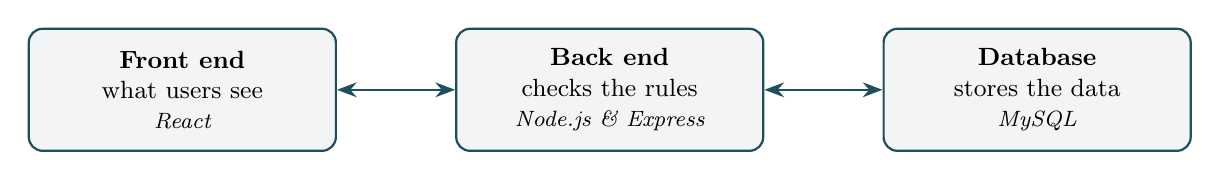
\begin{tikzpicture}[
  box/.style={draw=primary, rounded corners=5pt, thick, fill=primary!6,
              minimum width=3.9cm, minimum height=1.55cm, align=center, font=\small},
  arr/.style={{Stealth[length=2.5mm]}-{Stealth[length=2.5mm]}, thick, primary}
]
  \node[box] (fe) {\textbf{Front end}\\ what users see\\ \footnotesize\itshape React};
  \node[box, right=1.5cm of fe] (be) {\textbf{Back end}\\ checks the rules\\ \footnotesize\itshape Node.js \& Express};
  \node[box, right=1.5cm of be] (db) {\textbf{Database}\\ stores the data\\ \footnotesize\itshape MySQL};
  \draw[arr] (fe) -- (be);
  \draw[arr] (be) -- (db);
\end{tikzpicture}
\caption{The three main parts of the system}
\label{fig:parts}
\end{figure}

The \textbf{front end} is the part that users see and click on in their web
browser. I built it with React, a popular tool for creating interactive web
pages. The \textbf{back end} runs on a server. It receives every request,
checks who the user is, applies the registration rules and then sends back an
answer. I wrote it in JavaScript using Node.js and Express. Finally, the
\textbf{database} stores all the information, such as students, courses,
classes, timetables and grades, in eight connected tables. I used MySQL for
this part.

To keep the system secure, every user must log in, and passwords are never
stored as plain text. In addition, I packaged all three parts with a tool
called \emph{Docker}, so that the whole system can be started with a single
command on any computer.

\subsection{My working process}
I organised the work into five stages:
\begin{enumerate}[leftmargin=1.6em]
  \item \textbf{Analysis (January).} I studied how registration works at my
        university and wrote down nine rules that the system must follow, for
        example ``a student cannot register for a full class''.
  \item \textbf{Database and back end (March).} I designed the database and
        built the back end, which contains all the rules.
  \item \textbf{Reorganisation.} As the project grew, I restructured the code
        so that the front end and the back end live in one well-organised
        project.
  \item \textbf{Front end.} I built the student and administrator websites
        and improved the design.
  \item \textbf{Deployment and documentation.} I prepared the system for
        installation with Docker and wrote installation and technical documentation.
\end{enumerate}
Throughout the project, I used Git, a version control tool, to save every step
of my work. This meant that I could always go back if I made a mistake.

% =========================== 5. CHALLENGES ===========================
\section{The Biggest Challenges}

Although many parts of the project were straightforward, two problems took
much more time and thought than I had expected.

\subsection{Challenge 1: the last seat}
Imagine a class with 40 seats, and 39 students have already registered. Now,
two students click \emph{Register} at exactly the same moment. In a simple
system, both requests ask the database ``Is there a free seat?'', both receive
the answer ``Yes, one seat'', and both students are accepted. As a result, the
class ends up with 41 students, which is clearly unfair and causes problems
for the lecturer.

At first, I did not even notice this problem, because it never happened when I
tested the system alone. However, after reading about how real registration
systems work, I realised that it would definitely happen on a busy
registration day. To solve it, I used a database feature called a
\textbf{transaction with a lock}. In simple terms, when the first student starts
registering for a class, the system ``locks'' that class for a fraction of a
second. The second student has to wait until the first registration is
complete. When it is their turn, the system correctly sees that the class is
full and shows a polite message. In addition, I added a rule inside the
database itself, so that the number of students can never be higher than the
number of seats, even if there were a mistake in my code.

\subsection{Challenge 2: timetable clashes}
The second challenge was to stop students from registering for two classes
that take place at the same time. This sounds easy, but real timetables are
more complicated than they look. Some classes, for instance, only meet in odd
weeks, while others only meet in even weeks. I eventually defined a clear rule:
two classes clash only if \emph{all three} of the following are true:
\begin{itemize}[leftmargin=1.6em]
  \item they are on the same day of the week;
  \item their lesson periods overlap;
  \item their weeks are compatible (an odd-week class never clashes with an
        even-week class).
\end{itemize}
Whenever a clash is found, the system does not simply say ``Error''. Instead,
it tells the student exactly which of their classes is causing the problem, so
they know what to change.

% =========================== 6. WHAT I LEARNED ===========================
\section{What I Learned}

This project taught me much more than any single course exercise. On the
technical side, I became confident with all three parts of a web application,
and I now understand why reliability problems like ``the last seat'' matter so
much in real systems. More importantly, however, I developed several skills
that I believe will be useful in any job.

\begin{itemize}[leftmargin=1.6em]
  \item \textbf{Planning before acting.} Writing down the nine rules before
        coding saved me a great deal of time, because I always knew exactly
        what I was building.
  \item \textbf{Learning independently.} Many solutions, such as the
        transaction lock, were not taught in my classes. I had to find
        information in documentation and articles, most of which were written
        in English.
  \item \textbf{Writing clearly.} I wrote documentation so that other people
        could install and use the system. This taught me to explain technical
        ideas in simple, well-organised language, which is also the aim of
        this report.
  \item \textbf{Managing my time.} Breaking the work into stages helped me to
        make steady progress and to stay motivated.
\end{itemize}

If I had more time, I would like to add automatic tests, a waiting list for
full classes with email notifications, and an automatic check that students
have completed the required prerequisite courses.

% =========================== 7. CONCLUSION ===========================
\section{Conclusion}

In conclusion, the Course Management and Registration System is the project I
am most proud of so far. It started from a problem that I experienced myself
as a student, and it became a complete system that is fair, easy to use and
easy to install. Along the way, I faced real challenges, such as protecting the
last seat in a class and detecting timetable clashes, and solving them taught
me to plan carefully, learn independently and communicate clearly. Above all,
this project showed me that good software is not only about writing code, but
about understanding people's problems and solving them in a reliable way.

\end{document}
